\documentclass[AMA,STIX1COL]{WileyNJD-v2}
\usepackage{subcaption}
\usepackage{amsmath,amssymb,color}
\usepackage{graphicx}
\usepackage{lineno,etoolbox}
\newcommand{\linenomathpatch}[1]{%
  \cspreto{#1}{\linenomath}%
  \cspreto{#1*}{\linenomath}%
  \csappto{end#1}{\endlinenomath}%
  \csappto{end#1*}{\endlinenomath}%
}
\linenomathpatch{equation}
\linenomathpatch{gather}
\linenomathpatch{multline}
\linenomathpatch{align}
\linenomathpatch{alignat}
\linenomathpatch{flalign}
\newtheorem{example}[theorem]{Example}

\articletype{Research Paper}%

\received{\today}
\revised{}
\accepted{}
\linenumbers


\raggedbottom
\usepackage{hyperref}

\begin{document}

\title{On Water Wave Dynamics Using Physics Informed Neural Networks} 

\author[1]{Waasif Nadeem}

\author[2,3]{Volker John}

\author[1]{Zahra Lakdawala}

\authormark{AUTHOR ONE \textsc{et al}}


\address[1]{\orgdiv{Lahore University of Management Sciences}, \orgname{Department of Mathematics, School of Science and Engineering}, \orgaddress{\state{Lahore}, \country{Pakistan}}}

\address[2]{\orgdiv{Weierstrass Institute for Applied Analysis and Stochastics}, \orgname{Leibniz Institute in Forschungsverbund Berlin e. V. (WIAS)}, \orgaddress{\state{Berlin}, \country{Germany}}}

\address[3]{\orgdiv{Freie Universit\"at of Berlin}, \orgname{Department of Mathematics and Computer Science}, \orgaddress{\state{Berlin}, \country{Germany}}}

\corres{Zahra Lakdawala. \email{zahralakda@gmail.com}}

%\presentaddress{This is sample for present address text this is sample for present address text}

\abstract[Summary]{A vanilla feed forward neural network consists of neurons and layers and the mapping between input and output is approximated using a non linear function. The network is conventionally trained using data. In this work, we set up a neural network such that the spatio-temporal solution of time-dependent wave propogation models is learnt. This is done by providing the physical model, such as the 1D wave and shallow water wave equations and its associated boundary and initial conditions, as rules for learning the network. We invesitage the feasibility of data-driven and model-driven network predictions against numerical solutions. We  further investigate the accuracy of the trained network through different parameter configurations and look closely into the multi-objective loss function that is constructed by including the residual error of the physical equations and the associated initial and boundary conditions. We present the results of numerical solutions against solutions obtained from data and model-driven neural network using data and physics informed rules for learning. Lastly, we construct a hybrid data and physics driven network and show that this significantly improves the accuracy of the physics-driven network.}

\keywords{Physics informed neural networks, wave equation, data trained network, model-based learning, neural network}



\maketitle

\section{Introduction}

Partial differential equations (PDEs) are used to mathematically formulate the physical problems and hence, provide us with their solution. The physics of various real life applications comping from physics, biology, electrostatics, finance and other disciplines can be expressed in a complex system of PDEs. Our focus is to investigate the use of neural networks for predicting solutions for wave propogation models (acoustic wave equation and shallow water equation). In most real-scale models, it is either imposiible or infeasible to find an analytical solution for PDEs so we rely heavily on numerical schemes to find solutions. Numerical methods, however, can be very costly in terms of time and space and are proven to be quite inefficient for constantly changing environment. Efficient numerical computation has become increasingly important in this field. The solution is usually sought using one of the classical numerical methods such as Finite Difference, Finite Volume, Finite Element, etc.
\par
\noindent
In the past decade, we have seen machine learning methods such as Gaussian Regression Method, Neural Networks and Deep Learning approaches achieve great results specially in the field of image processing and natural language processing. It has become a widely popular field of research to train machine learning algorithms with physical rules \citep{}. It has been shown \citep{} that if one trains a neural networks with appropriate physics, the engine can be used to predict solutions for complex systems of partial differential equations. A physics informed neural network (PINN) learns the solution to a PDE using the information regarding initial and boundary conditions of the equation in addition to the solution itself. The theory of neural networks state that it can learn any function but as the functions get complicated the number of layers needed to learn that function approaches infinity, which is not something we can apply in practice. PINNs learns the physics and the associated with much less layers than what is required for a conventional network. In addition, it is shown that PINN can also be used to predict solutions of PDEs with slight change in their initial conditions. The issue of efficiency, convergence and accuracy of solutions obtained from using PINNs is explored deeply \citep{}. Regarding this aspect, only a few studies illustrate how the changes in the neural network configurations affect the solution \citep{}, \citep{}. Even fewer report on how the optimization functional can be modified for various physics to get better convergence and accuracy. 
\par
\noindent
This work focuses towards employing neural networks and deep learning frameworks to as an alternative method for finding  solutions of such partial differential equations. We consider the 1D wave equation and 1D Shallow Water Equation (SWE) along with its associated initial and boundary conditions as physical rules to train a neural network. We employ three ways of training the neural networks i) using data from numerical solutions; ii) using only the model/physics as given by the physical equation and its associated initial and boundary conditions; iii) using a hybrid approach that combines both the data and physical model to train the network.  
\par
\noindent
This paper is organised as follows: we first provide a short introduction to the 1D wave and shallow water models considered as the physical models for training of PINNs. This is followed by a description of a vanilla feed forward neural networks. We constructa multi-objective loss function for optimizing the hyperparameters of the network. We further discuss a worked out a worked out example for how the loss function is modified to incorporate the physical model at hand. Section \ref{sec:results} shows the solution and evolution plots for data and physics trained neural networks and compares them against  reference(numerical) solutions. We draw out a detailed discussion of the results in Section \ref{sec:conclusion} summarizing our work and findings.


\section{The considered initial-boundary value problems}
Waves are very important in the field of fluid dynamics,
acoustics, and many other physical problems as they are an effective way to transmit information (sound, fluid, etc.) across several spatio-temporal scales. 
Our focus is mainly on hydrological applications, however the results can be informative for anyone studying wave dynamics. We focus on two models that describe wave dynamics, namely the 1D acoustic wave and shallow water equations. 
 
\subsection{Wave equation}

A wave equation, modeling the propagation of a wave at a fixed speed is defined as:
\begin{equation}
\label{eq:wave}
\frac{\partial^2u}{\partial t^2} = c^2 \frac{\partial^2u}{\partial x^2},\quad \mbox{where } x \in [x_0, x_{\mathrm{end}}], t \in (0, t_{\mathrm{end}}].
\end{equation}
Here, $u(x, t)$ is the displacement in the second space dimension ($y$-direction) and $c$ is the velocity of wave. The equation is equipped the initial and boundary conditions
\begin{equation}
\label{eq:wave_cond}
u_0 = u(x,0) = u_{\mathrm{in}}(x), \quad
\left.\frac{\partial u(x, t)}{\partial t} \right|_{t=0} = u^{\prime}_{\mathrm{in}}(x), \quad 
u(x_0, t) = u(x_{\mathrm{end}}, t). 
\end{equation}

\subsection{Shallow water equation}

Shallow water equations (SWE) are a set of equations that are derived from physical conservation laws for mass and momentum to describe fluid flow problems. They can be derived by depth averaging 
the Navier--Stokes equations. They are used in predicting cyclones, storm surges, flows around structures etc..

For simplicity, the 1D SWE is used in our study of deep learning techniques. 
This equation is derived from the 2D equations of mass and momentum conservation based on assumption
of incompressibility of water, hydrostatic pressure distribution, and a sufficiently small channel slope. 
The conservative form of 2D SWE takes the following form   
\[
\frac{\partial}{\partial t}Q + \frac{\partial }{\partial t} F(Q) + \frac{\partial }{\partial t} G(Q) = 0,
\]
where $u$ and $v$ are the depth-averaged water velocity in $x$ and $y$ directions, $h$ is the water height 
with respect to a bottom profiled domain as a zero line, and 
$Q = (h, hu, hv)^T$, $F(Q) = (hu, hu^2+ \frac{1}{2}gh^2, huv)^T$, $G(Q) =(hu, huv, hu^2+ \frac{1}{2}gh^2)^T$.
This equation has to be equipped with appropriate initial and boundary conditions. 


The 1D SWE, after having differentiated the terms using the product rule, is written as
\begin{equation}\label{eq:swe}
\begin{array}{rcll}
\displaystyle\frac{\partial h }{\partial t} + u \frac{\partial h }{\partial x} + h \frac{\partial u }{\partial x}  &=& 0
& \mbox{with } x \in [x_0, x_{\mathrm{end}}], t \in (0, t_{\mathrm{end}}],\\[1em]
\displaystyle  h \frac{\partial u }{\partial t} + u \frac{\partial h }{\partial t}  + u^2 \frac{\partial h }{\partial x} + 2uh\frac{\partial u }{\partial x} + g \frac{\partial h }{\partial x} &=& 0 & \mbox{with } x \in [x_0, x_{\mathrm{end}}], t \in (0, t_{\mathrm{end}}],\\[1em]
\end{array}
\end{equation}
where $h$ is the water depth and $u$ is depth-averaged velocity. Hence, in contrast to the wave equation, 
the solution of the 1D SWE is vector-valued. The initial  and boundary 
conditions are given by 
\begin{equation}\label{eq:swe_ic_bc}
u_0 =  u(x,0), \quad  h_0 = h(x,0),\quad 
u_{x_0}=u(x_0,t), \quad  u_{x_{\mathrm{end}}} = u(x_{\mathrm{end}}, t) . 
\end{equation}

We consider the parameterized form of the wave equations described above. A n-th order  partial differential equation along with its initial and boundary conditions can be written as: 
\begin{eqnarray}
  \label{eq:pde}
 \mathcal{F}_{PDE}\left(u, \frac{\partial u}{ \partial t}, \frac{\partial u}{ \partial x}, \frac{{\partial}^2 u}{\partial x^2}, \ldots, \vec{\nu}\right) &=&0 \;  \mbox{for } x \in \Omega, t \in (0,T],\\
\label{eq:ic}
  \mathcal{F}_{IC}\left(u, \frac{\partial u}{ \partial t}, \frac{\partial^2 u}{ \partial t^2}, \ldots\right) &=& 0 \;
 \mbox{for } x \in \Omega \cup \bar{\Omega}, t = 0,\\
\label{eq:bc} \mathcal{F}_{BC}\left(u, \frac{\partial u}{ \partial x}, \frac{\partial^2 u}{ \partial x^2}, \ldots   \right) &=&0 \;  \mbox{for } x \in  \bar{\Omega}, t \in (0,T], 
\end{eqnarray}
where $\Omega$ and $\bar{\Omega}$ denote the spatial domain and its boundary,respectively. 
Here, $\mathcal{F}_{PDE}$ describes the differential operators and $\vec{\nu} = (\nu_1, \nu_2, \ldots)$ 
denotes the parameters of the partial differential equation. We seek to find the solution $u(x,t)$ of the initial-boundary value 
problem with initial conditions and boundary conditions denoted by $\mathcal{F}_{IC}$ and $\mathcal{F}_{BC}$ respectively. 
\section{Data driven and physics informed neural networks}
\label{sec:neuralnets}
This section reviews a data driven neural network(DDNN) and physics informed neural network(PINN) in the context of seeking solutions for the acoustic and shallow water wave equations \ref{eq:wave}-\ref{eq:swe}. Only a few studies have discussed a hybrid neural network (HNN) that combines data-driven and phyics informed neural networks. We introduce the hybrid approach for the wave equations and discuss the composition of loss function in each of the approaches in detail.

\subsection{A data-driven neural network (DDNN)}
\label{sec:vanillaNN}
A simple forward feed convolutional neural network, denoted by $U(x, t, u^*); \theta)$, can generally be described by three components, namely  multiple layers consisting of neurons and a global architecture. If the weight $w_{jk}^l$ connects the $k$-th neuron in the ($l-1$)th layer to the $j$-th neuron in the $l$-th layer, the relationship for the output $\tilde{u}_j^l$ can be written as
\[
\tilde{u}_j^l = \sigma\left(\sum_k w^l_{jk} \tilde{u}_k ^{l-1} + b_j^l\right) =  \sigma\left(z_j^l\right).
\]
Each neuron of a layer is connected to each neuron of the next layer and is associated with a weight, a bias term, and an activation function. The  activation function is applied to a signal at evey layer before it is passed to the next layer. For example, a sample input $x$ with a sigmoid activation function sees a transformation of $\sigma(x) = \frac{1}{1+e^{-x}}$ when it meets the next layer. The choice of the activation function will be one aspect in our studies. The choice is usually determined by certain factors such as explosion or vanishing gradients, making clear predictions, and/or computational efficiency.
%
The feed forward network uses the principle of back propogation to address how a variation in weight and biases impact the output error. Simply put,the network parameters $\theta$ (weights and biases) are found using an optimization routine such that the resulting output is close to the desired target solution. Here is where a loss function forms the crux of the training of the network. In a supervised regression problem, the output loss is often the mean squared error (MSE) computed using the difference of the actual output value and the desired target value $u(x,t)$:
\begin{equation}\label{eq:fct_data}
\mathcal{L}_{\mathrm{data}}= \frac{1}{N} \sum_i^N \left\| u(x_i,t_i) - \tilde{u}(x_i,t_i) \right\|_2^2,
\end{equation}
where  $N$ is the number of uniformly sampled collocation points defined 
as the data set $\{ x_i,t_i \}, i \in \{1, \ldots, N\}$.  The output $\tilde{u} = \tilde{u} (x, t, \theta)$ is
expressed as a function of the input $(x, t)$ and the network parameters $\theta$. The training process aims to find $\theta$, given the input $(x, t, u^*)$, by solving the following optimization problem 
\[
\mbox{argmin}_\theta \mathcal{L} \left(\theta\ | \ (x,t ,u^*)\right),
\]
where the function $u$ maps $(x, t)$ to measurements/true solution at those coordinates. A neural network needs an optimization routine to update its weights and biases in the direction of minimizing a loss function defined on the output. This routine is generally a (stochastic) gradient descent algorithm or a quasi Newton method.  The training is complete once the network has found parameters such that a desired accuracy of the loss function is reached. The learnt function is based just on the training input data $u^*$ and $(x,t)$. We will talk about the training data in detail later in Section \ref{sec:hnn}. 

\subsection{Physics informed training of the neural network}
\label{sec:pinns}

If one is interested in finding the solution of an initial-boundary value problem, then it seems to be a quite natural idea to incorporate this problem into the loss function, i.e. the physics instead of data. The physical model comprises of differential equations,along with its boundary and/or initial conditions. The problem is defined on a spatial and/or temporal domain. The  parameterized form of the problem is considered, as shown in equations \ref{eq:pde} -  \ref{eq:bc}. Let us denote the neural network by   
$U(x, t, \theta )$ and the function learnt by the network is the solution to the physics model, denoted by $\tilde{u}(x,t)$. 
In PINNs,  the residuals of the partial differential equation, initial, and boundary conditions are included, 
where we used the $L^2$-norm $\|\cdot\|_0$  (mean squared error / MSE) on uniformly sampled collocation points prior to training,    

The PINNs with space and time coordinates as described in \cite{??} consist of a multiple dense layers, with weights and biases as described in Section~\ref{sec:vanillaNN}, along with a gradient layer. The derivatives of the output of the vanilla neural network, $u$, are used for calculating the strong residuals of the 
partial differential equation. The norm of these residuals, together with norms of residuals for 
initial and boundary conditions, are part of the loss functions. The loss function, which uses only
the physics-based information is defined  by 
\begin{equation}\label{eq:fct_phys}
\mathcal{L}(\theta, \nu ) = \mathcal{L}_{\mathrm{PDE}}  + \underbrace{\mathcal{L}_{\bar{\Omega}_1} + \ldots  + \mathcal{L}_{\bar{\Omega}_n}}_{= \mathcal{L}_{\mathrm{IC}}}  + \underbrace{\mathcal{L}_{\Theta_1} +\ldots + \mathcal{L}_{\Theta_m}}_{= \mathcal{L}_{\mathrm{BC}} },
\end{equation}
with \textcolor{red}{Is it correct that $\mathcal{L}_{\mathrm{data}}$ belongs 
to this functional? Shouldn't it appear only in the hybrid NN?}
\[
\mathcal{L}_{\mathrm{PDE}} = \frac{1}{|\tilde{\Omega}|} \sum_{x,t \in \tilde{\Omega}} \| \mathcal{E}\|^2_0, \quad
\mathcal{L}_{\mathrm{IC}} = \frac{1}{|\tilde{\Theta}|} \sum_{t \in \Theta_i} \| \mathcal{I}\|^2_0, \quad  
\mathcal{L}_{\mathrm{BC}}  = \frac{1}{|\tilde{\Gamma}|} \sum_{t \in \Gamma_i} \| \mathcal{B}\|^2_0.
\]
\textcolor{red}{There are a number of undefined symbols included. Do we need them?}
DDNN used a single objective loss function,whereas  PINNs find the training parameters by minimizing a multi-objective loss functional $\mathcal{L} (\theta, \nu)  = \sum_{i=1}^k \mathcal{L}_i ( \theta , \nu)$.
The training process solves the following optimization problem 
\[
\mbox{argmin}_\theta \mathcal{L} (\theta, \nu \ | \ (x,t ,physics)).
\]

%In this way, a neural network is created in the first step of training, using $(x,t)$ as input
%and with output $\tilde{u}$. 
PINNs use the gradient layer and take the whole data driven network as an input, so that the result of the 
gradient layer provides derivatives of the approximation to the solution
of the partial differential equation predicted by the network. 


\begin{example}[Wave equation] 
The following loss function shall enforce the network to compute an approximation $\hat{u}(x,t) =  U(x,t, \theta)$ 
of the solution $u(x,t)$ of the initial-boundary value problem for the wave equation 
\eqref{eq:wave}, \eqref{eq:wave_cond}:
\begin{eqnarray*}
\mathcal{L} &=& \underbrace{ \frac{1}{|\Omega |}  \sum_{(x,t) \in \Omega}
\left\| \frac{\partial^2 U(x,t, \theta)}{\partial t^2} - c^2 \frac{\partial^2 U(x, t, \theta)}{\partial x^2}\right\|_0^2}_{\mathcal{L}_{\mathrm{PDE}}} 
+ \underbrace{\frac{1}{|\tau_1|}  \sum_{(x,t) \in \tau_1} \left\| U(x_0, t, \theta) \right\|_0^2}_{\mathcal{L}_{\tau_1}} + \underbrace{\frac{1}{|\tau_2|}  \sum_{(t, x) \in \tau_2} \| u(x_{\mathrm{end}},t, \theta) \|_0^2}_{\mathcal{L}_{\tau_2}} \\
&&+ \underbrace{\frac{1}{|\gamma_1|}  \sum_{x \in \gamma_1} \| U(x, 0, \theta) - u_{\mathrm{in}}(x) \|_0^2}_{\mathcal{L}_{\gamma_1}} + \underbrace{\frac{1}{|\gamma_2|}  \sum_{x \in \gamma_2} \left\| \frac{\partial U(x, 0, \theta)}{\partial t} - u^{\prime}_{\mathrm{in}}(x) \right\|_0^2}_{\mathcal{L}_{\gamma_2}}.
\end{eqnarray*}
\textcolor{red}{This is not clear. 
\begin{itemize}
\item Do we take the $L^2$ norm in the space time domain? Then we do not need to sum anything. 
\item Do we take the $L^2$ norm only in space? Then we have to sum over the time steps.
\item Or do we use an $l^2$ norm for the vector? Then we need to sum. A number of symbols have to be 
introduced.
\end{itemize}
Such notations like $(x,t) \in \Omega$ are wrong. 
}
\end{example}
\subsection{Hybrid Neural neutwork}
\label{sec:hnn}

\subsection{Neural networks and optimization of hyperparameters}

The effects of using different architectures of the neural networks with respect to the number of layers 
and nodes per layer were investigated in preliminary studies. We found that the impact of these parameters 
on the aspect we are most interested in, namely the predictions for unseen situations, was only weak. 
For the sake of brevity, we will present results only for a network with $6$ deep (dense) layers containing $[128, 64, 32, 32, 64, 128]$ nodes, respectively. This is the ame configuration that was used in 
\cite{??}. \textcolor{red}{you said that there is some other paper which uses the same network}

Our preliminary studies also showed that the choice of the activation function might considerably influence the 
quality of the predictions from the neural networks. In Section~\ref{sec:results}, results obtained 
with different activation functions will be presented: $\tanh(x)$, 
\textcolor{red}{at least two more activation functions}

The library \textsc{TensorFlow} \cite{tensorflow2015-whitepaper} was used for constructing the neural networks and for solving the optimization problems. 
The optimization problems were solved with the 
limited-memory BFGS (L-BFGS) alogrithm  \cite{NW06}. This popular method is a  quasi  Newton method, which approximates the 
Hessian on the basis of  a prescribed maximal number of previous iterates.
\textcolor{red}{number of vectors used in the numerical simulations, initial value for optimization}


\section{Results}
\label{sec:results}
We have considered one test case for the wave equation \ref{eq:wave} with a known solution, and two test cases for shallow water equation \ref{eq:swe} to investigate the results from three neural networks described in section \ref{sec:neuralnets} . We investigated several aspects: 1) the  forward problems and accuracy of solutions learnt from each of the neural network with respect to analytical/reference solutions of the pdes; 2) the convergence of the optimizater with respect to the multiobjective loss function; 3)  we provide a few insights on whether neural netwrks can be a reliable long term prediction algorithm based on limited training data. 
\par
We studied the impact of different layered architectures of the neural netwrok ranging from 6 to 24 hidden layers, with different configurations of nodes in every layer ranging from 8 to 64 nodes. Increasing the number of hidden layers and the node confugrations seemed to have almost no impact on the quality of solutions. We also studied the the impact of using different activation functions, and only tanh activation function seemed to work for the three cases. For the sake of brevity, only selected and representative results are included. 

\subsection{Wave equation}
\label{subsec:wave_res}
We consider equation \eqref{eq:wave} for $x \in [0,1]$, $t \in [0,1]$, and $c =1$.  A solution of this 
equation is given by 
\[
u(x,t) = \frac{1}{2} \sin (\pi x) \cos(\pi t) + \frac{1}{3} \sin (3\pi x) \sin (3 \pi t).  
\]
This function is for the boundary conditions a $u(0,t) = u(1,t) =  0$ and the initial 
conditions 
\[
u_0  = u(x,0)  = \frac{1}{2} \sin (\pi x), \quad u_0^{\prime}=\frac{\partial u}{\partial t}(x,0) = \pi  \sin (3 \pi x)
\]
the solution of the initial-boundary value problem \eqref{eq:wave} -- \eqref{eq:wave_cond}.

We use the numerical solution using a finite difference method. The training for PINNS , DDNN and HNN uses 100 $(x,t)$ tuples of uniformly sampled points on the grid for $ x\in (0,1)$ and $t \in (0,0.8]$,  another 100 $(x,t)$ tuples on the boundary $x =0$, $x=1$ and another 100 tuples each for the initial conditions $u_0$ and $u_0^{\prime}$ . DDNN further uses the tuple $(x,t, u(x,t))$ including the solution of the PDE evaluated at the sampled grid points as part of training data. PINN further includes the PDE evaluation of $u$ on 100 $(x,t)$  tuples (in the domain interior) as part of the loss functional. The gradient terms in the PDS are evaluated using automatic differentiation in TensorFlow.  HNN training was done using $100$ randomly selected tuples of $(x, t, u(x,t))$  and PDE evaluation of $u$ as part of the loss functional .The configuration for all the three networks consisted of 4 layers with 32 nodes in each layer using $tanh$ activation function.
\par
The formulation of loss functionals are different for each of the networks, as described in Section~\ref{sec:neuralnets}. Figure~\ref{fig:wave_loss_contributions} illustrates how the each of the residual terms in \eqref{eq:loss} is minimized in the multi-objective optimization routine. Moreover, we see that the convergence and estimation of hyperparameters requires around . However, the performance for PINN  in this case is quite satisfactory given no pre-computed solutions are required to train the network.   
\textcolor{red}{the pictures need more explanations. I do not understand that the overall loss 
is smaller than the largest individual loss.}
\begin{figure}[t!]
\begin{center}
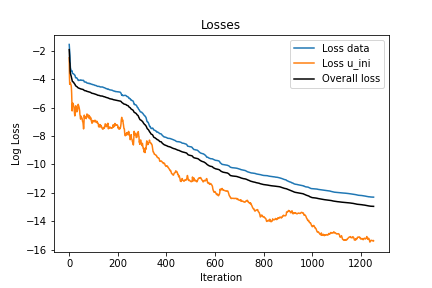
\includegraphics[width=0.45\linewidth]{../Code/B1/losses/combined_losses_reduction_data.png}
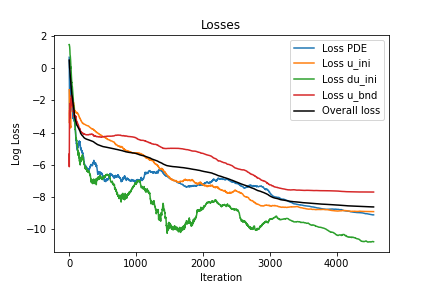
\includegraphics[width=0.45\linewidth]{../Code/B1/losses//combined_losses_reduction_PINNs.png}
\end{center}
\caption{Wave equation. Activation function $\tanh(x)$. Convergence of the optimization process 
for minimizing the loss functionals and their individual terms. Note the different scaling of the 
abscissa.}\label{fig:wave_loss_contributions}
\end{figure}


The hyperparameters were used to predict solutions for $t \in [0,0.8]$ to see if solution was correctly learnt using the training data. We also used the same network to predict the solution for $t \in [0.8,1.0]$.

\begin{figure}[t!]
\begin{center}
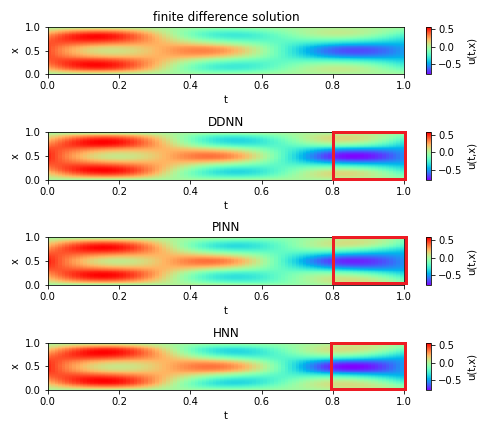
\includegraphics[width=0.4\linewidth]{../Code/B1/plots/colormap.png}
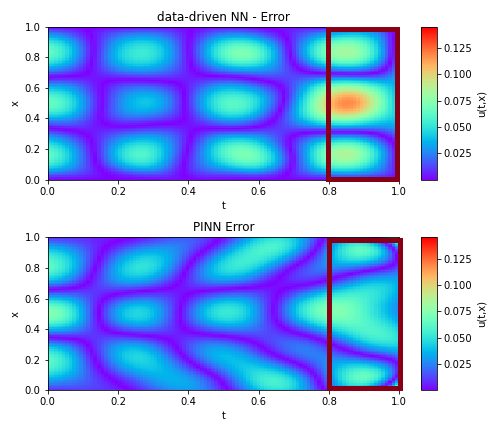
\includegraphics[width=0.3\linewidth]{../Code/B1/plots/error_colormap.png}
\end{center}
\caption{Left: Solution $u(x,t)$ obtained from FD numerical scheme, PINN and HNN. Right: The error maps for PINN, DDNN and HNN}
\label{fig:wave_sol_error}
\end{figure}

Figure~\ref{fig:wave_sol_error} (left) shows the comparison of the results of the 
data- and physics-driven neural networks to the finite difference solution. 
In the right-hand side pictures the error maps for both networks are depicted, where the 
(abolute value of the) error in each node in space and time was computed. 
Whereas the errors in $t\in[0,0.8]$ are of the same size for both networks, at most of the order $0.075$,
it can be seen that the PINNs performed better than the data-trained network for $t\in[0.8,1]$.
\textcolor{red}{Before, the sentence was the other direction. I changed in it accordance with the labels 
of the pictures.}

\begin{figure}[t!]
\begin{center}
%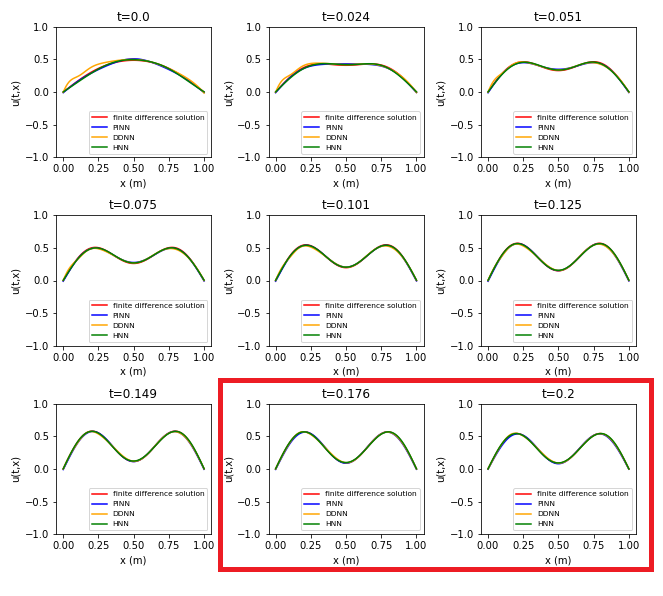
\includegraphics[width=0.45\linewidth]{../Code/B1/plots/wave_numerics.png}
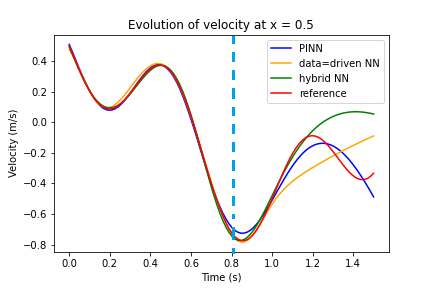
\includegraphics[width=0.45\linewidth]{../Code/B1/plots/evolution_plot.png}
\end{center}
\caption{Left: Convergence of the optimizer using the loss functionals for DDNN, PINN and HNN. Right: Temporal evolution of velocity at $x=0.5$ for longer time period $t\in [0,1.5]$.}
\label{fig:wave_evolution}
\end{figure}

Figure~\ref{fig:wave_evolution} presents more information on the prediction of the wave velocity. 
In addition to using all time steps in $[0,0.8]$ for learning the data-driven network, also the 
case of using only every $4$th time step. One can observe that in $[0,0.8]$ the predictions 
from all networks are quite similar. However, there are differences for the unseen situation.
The data-driven network lead to predictions with a much larger error in the middle of the interval for $t=0.879$. And for longer time horizons, $t>1.2$, the PINN prediction is significantly more reliable.
\textcolor{red}{To be honest, I do not see the new information of the left picture.}


\subsection{Shallow water equation}

The initial boundary value problem \eqref{eq:swe} -- \eqref{eq:swe_ic_bc} for the shallow water 
equations was solved in $(x,t) \in [0,1]\times [0,0.2]$. The velocity is considered to be at equilibrium at $t=0$, i.e. $u(x, 0) = 0$.
Two different initial profiles for 
$h(x,0)$ will be considered, leading to solutions with different features.
\textcolor{red}{provide 
information about compuation of the solution to compare with: discretizations in time and space, 
finenss}

Besides the data-driven neural network and the PINN, we will study for this example also a hybrid network, where the loss functional is the following linear combination of the data part \eqref{eq:fct_data} and the physics part \eqref{eq:fct_phys} \textcolor{red}{give concrete linear combination}
All networks will be trained with the numerical solution from $[0,0.15]$ and the unsee situation 
is the solution in $(0.15,0.2]$. 


  
\subsubsection{Initial profile $h(x, 0)$ leading to a smooth solution}

\begin{figure}[t!]
\begin{center}
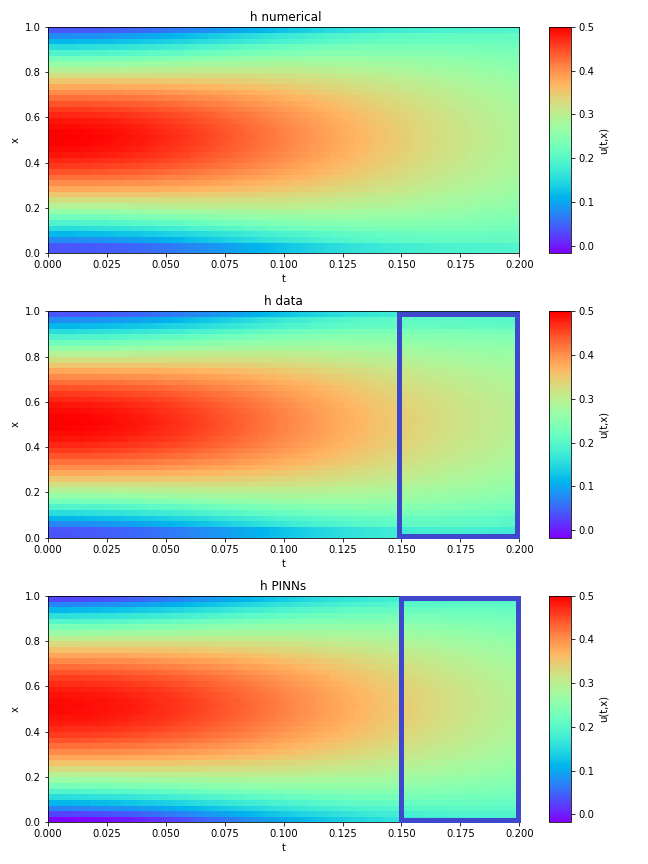
\includegraphics[width=0.45\linewidth]{./plots/h_colormap_b1.png}
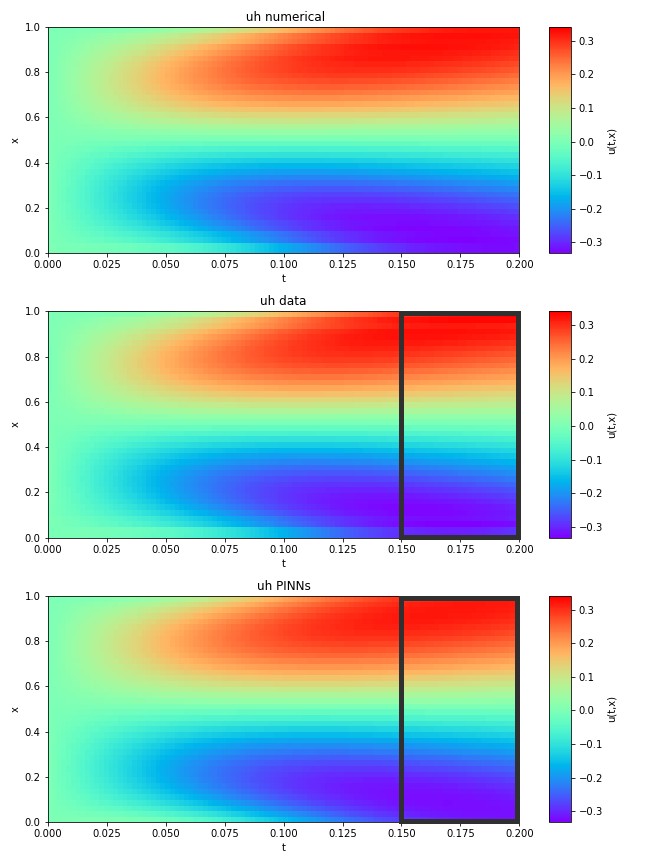
\includegraphics[width=0.45\linewidth]{./plots/uh_colormap_b1.png}
\end{center}
\caption{Shallow water equations, smooth solution. ctivation function $\tanh(x)$. Solution of 
the initial boundary value problem (top), solution obtained with the data-driven neural network (middle), 
solution obtained with the PINN (bottom).}
\label{fig:b1_swe_sol}
\end{figure}

The initial profile of the height considered in this example has the form  $h(x,0) =\frac{1}{2} \sin (\pi x)$.
The numerical solution of  \eqref{eq:swe} -- \eqref{eq:swe_ic_bc} can be seen in the upper part of 
Figure~\ref{fig:b1_swe_errors}.

\begin{figure}[t!]
\begin{center}
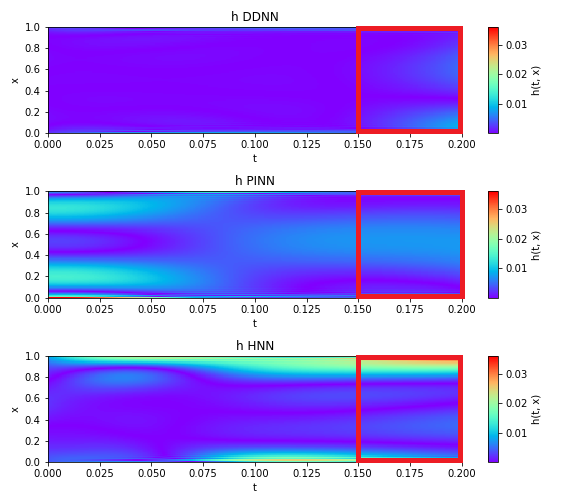
\includegraphics[width=0.45\linewidth]{../Code/B2/plots/h_errorplot_b1.png}
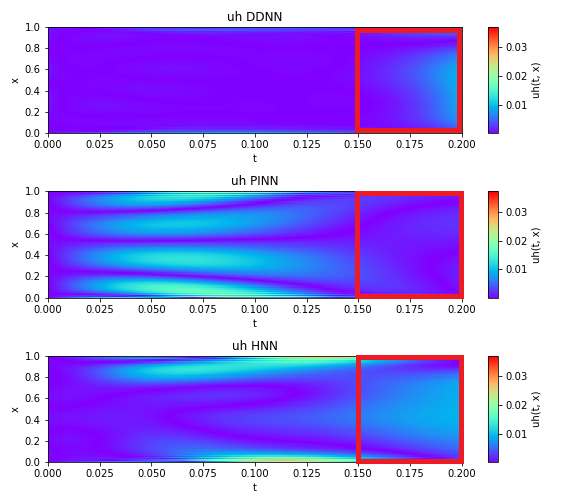
\includegraphics[width=0.45\linewidth]{../Code/B2/plots/uh_errorplot_b1.png}
\end{center}
\caption{
Error maps of $h(x, t)$ and $u(x,t)$ for the data driven neural network (left) and the PINN (right).}\label{fig:b1_swe_errors}
\end{figure}

Comparisons of the results obtained with the data-driven neural network and the PINN are presented
in this picture as well and the corresponding errors in Figure~\ref{fig:b1_swe_errors}. For the 
seen interval $[0,0.15]$, the results with the data driven neural network are clearly 
more accurate. This situation changes somewhat for the unseen interval, where the velocity error
for the data driven network becomes large at the left spatial boundary and $t\to 0.2$. But altogether, 
one can conclude that both neural networks give satisfactory results for $t\in[0,0.2]$


\begin{figure}[t!]
\begin{center}
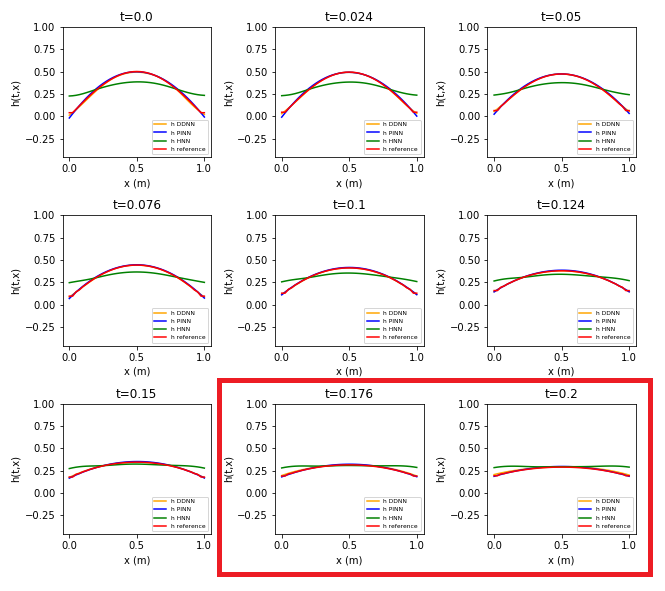
\includegraphics[width=0.45\linewidth]{../Code/B2/plots/h_b1.png}
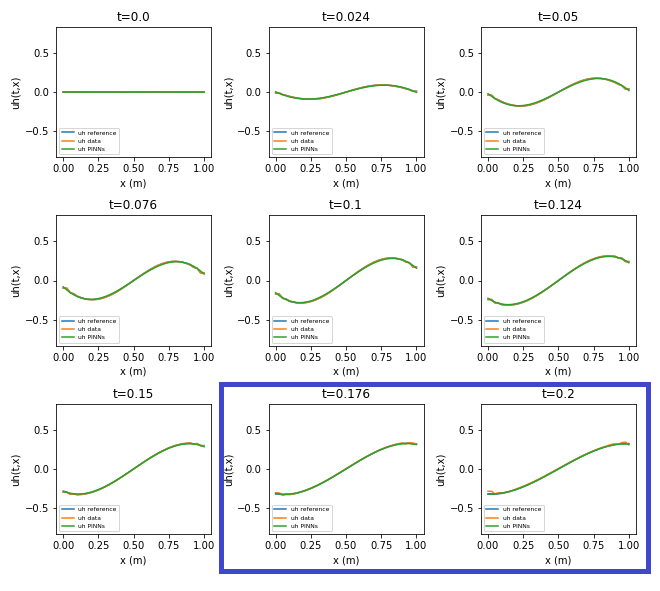
\includegraphics[width=0.45\linewidth]{../Code/B2/plots/uh_b1.png}
\end{center}
\caption{Shallow water equations, smooth solution. ctivation function $\tanh(x)$.  Solutions $h(x, t)$ and $u(x,t)$ plotted at different $t$.
\textcolor{red}{Do we need this picture? What are the new information?}}\label{fig:b1_swe_time}
\end{figure}


\begin{figure}[t!]
\begin{center}
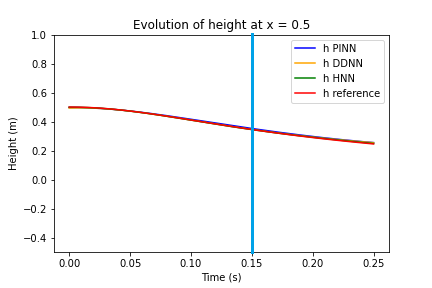
\includegraphics[width=0.45\linewidth]{../Code/B2/plots//h_evolution_plot_b1}
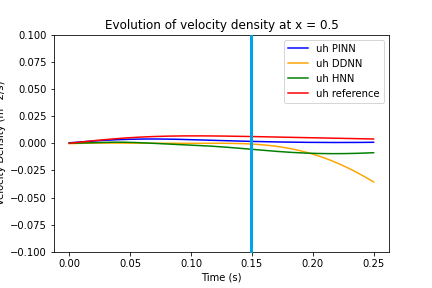
\includegraphics[width=0.45\linewidth]{../Code/B2/plots/uh_evolution_plot_b1}
\end{center}
\caption{Shallow water equations, smooth solution. ctivation function $\tanh(x)$.  Solutions $h(x=0.5,t)$ and $u(x=0.5, t)$ forward-in-time predictions.}\label{fig:b1_swe_time_x05}
\end{figure}

However, extending the unseen time interval a little bit further, the prediction from the 
data-driven neural network becomes unreliable, compare Figure~\ref{fig:b1_swe_time_x05}.

\textcolor{red}{shall we present results for the hybrid network here, or just say that they are not 
much different, because the results for the other networks are not much different as well?}

\subsubsection{Initial profile $h(x,0)$ leading to a solution with shocks}

We solved the shallow water equation for a slightly more realistic dam flow example where the initial profile of $h(x,0) =2+sin (2\pi x) $ results in a more complex wave propogation. The velocity is considered to be at equilibrium at $t=0$, i.e. $u(x, 0) = 0$. 
\par
\noindent
The solutions are compared against the reference/numerical solutions in figure \ref{fig:b2_swe_sol}. Both data and physics driven network learn the solution within a $10^{-2}$ accuracy as can be seen in figure \ref{fig:b2_swe_errors}.
\par
\noindent
For feed forward predictions of the solution for the time that's not incorporated in the training, the hybrid approach works better than PINNs. It can be seen in figure \ref{fig:b2_swe_time} that when looked on a micro scale, data-driven network overestimates the predicted velocities. Overall, learning for both networks is quite satisfactory for the case of gradual propogation of the wave. 

\begin{figure}[t!]
\begin{center}
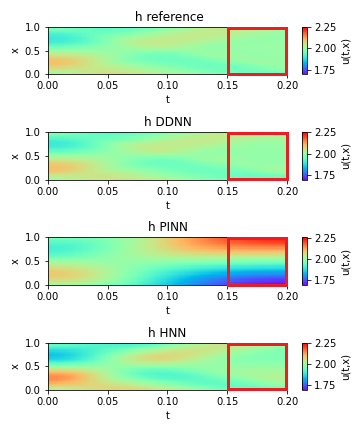
\includegraphics[width=0.45\linewidth]{../Code/B3/plots/h_colormap_b2.png}
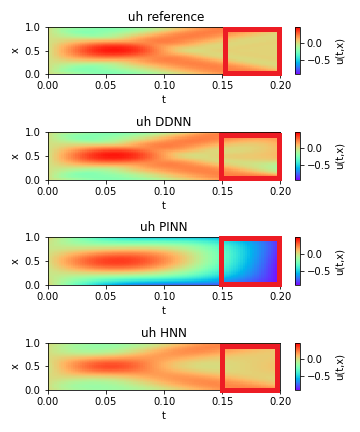
\includegraphics[width=0.45\linewidth]{../Code/B3/plots/uh_colormap_b2.png}
\end{center}
\caption{Case 2.2  Comparison of the $h(x,t)$ $and u(x,t)$ obtained from numerical, data and model-trained network}\label{fig:b2_swe_sol}
\end{figure}




\begin{figure}[h!]
\begin{center}
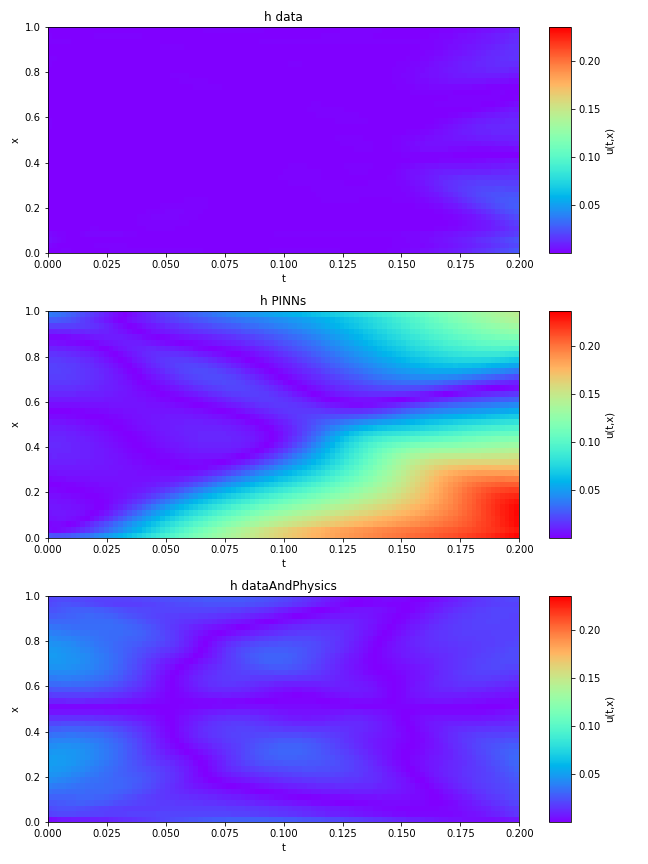
\includegraphics[width=0.45\linewidth]{../Code/B3/plots/h_errorplot_b2.png}
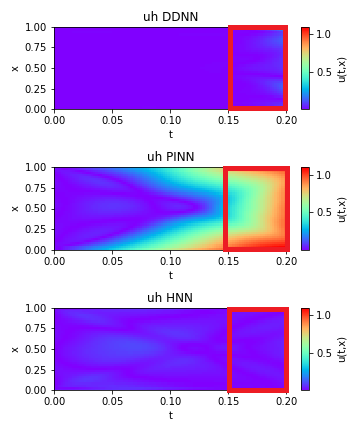
\includegraphics[width=0.45\linewidth]{../Code/B3/plots/uh_errorplot_b2.png}
\end{center}
\caption{Case 2.2: The error maps of $h(x, t)$ and $u(x,t)$ is plotted as a color map.}\label{fig:b2_swe_errors}
\end{figure}

\begin{figure}[h!]
\begin{center}
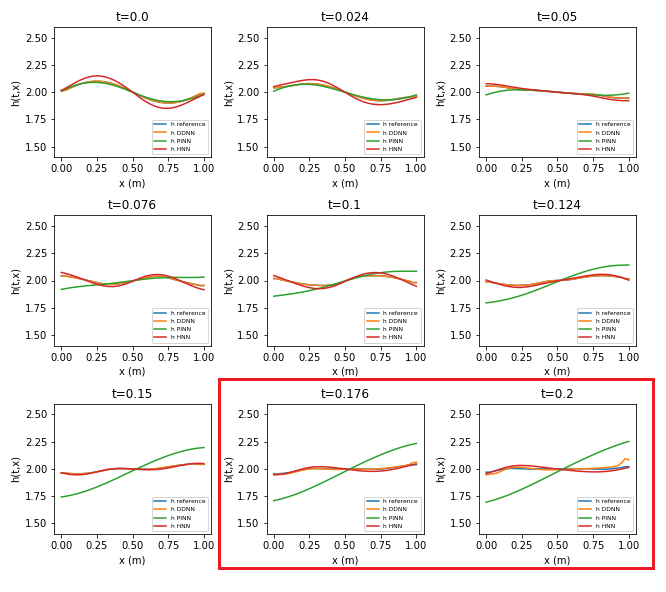
\includegraphics[width=0.45\linewidth]{../Code/B3/plots/h_b2.png}
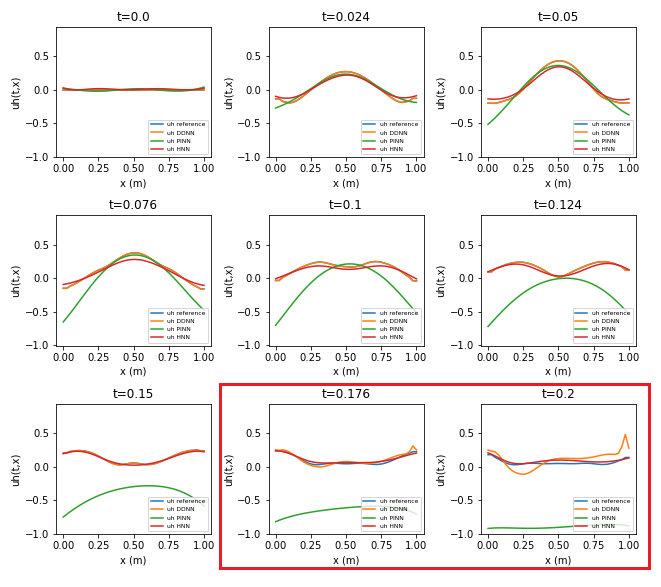
\includegraphics[width=0.45\linewidth]{../Code/B3/plots/uh_b2.png}
\end{center}
\caption{Case 2.2: Solutions $h(x, t)$ and $u(x,t)$ plotted at different $t$.}\label{fig:b2_swe_time}
\end{figure}


\begin{figure}[h!]
\begin{center}
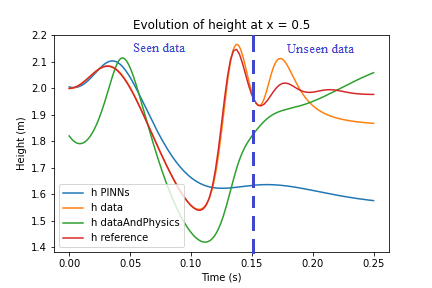
\includegraphics[width=0.45\linewidth]{./plots/h_evolution_plot_b2.png}
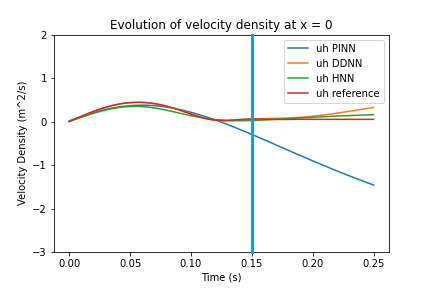
\includegraphics[width=0.45\linewidth]{../Code/B3/plots/uh_evolution_plot_b2.png}
\end{center}
\caption{Case 2.2: Solutions $h(x=0.5,t)$ and $u(x=0.5, t)$ forward-in-time predictions.}\label{fig:b2_swe_time_x05}
\end{figure}

\section{Conclusion}
\label{sec:conclusion}
Cant colnclude that PINNS works best for SWE. changing layer and node configuration hardly makes a difference in training the networks. In the case of smooth solutions of wave models, PINNs predicts velocity(density) and/or height rather accurately. However for more complex/coupled systems, data-driven networks seem to work better. However data-fed networks need exhaustive datasets (solutions of model equations). In the absence of exhaustive data for learning of complex solutions, a hybrid training is recommended. 




\section*{Conflict of Interest Statement}
%All financial, commercial or other relationships that might be perceived by the academic community as representing a potential conflict of interest must be disclosed. If no such relationship exists, authors will be asked to confirm the following statement: 

The authors declare that the research was conducted in the absence of any commercial or financial relationships that could be construed as a potential conflict of interest.

\section*{Author Contributions}
ZL developed the code base for physics informed deep learning neural networks and put the article together. WN trained, and evaluated the models. VJ reviewed and refined the results. All authors contributed to the article and approved the submitted version.
\section*{Funding}
We acknowledge support from the DAAD through grant awards. We thank DAAD for their support.

\section*{Acknowledgments}
We thank Prof. Muhammad Abubakr and Prof. Karsten Berns for helpful discussions at the early stage of this work.

\section*{Supplemental Data}
 \href{http://home.frontiersin.org/about/author-guidelines#SupplementaryMaterial}{Supplementary Material} should be uploaded separately on submission, if there are Supplementary Figures, please include the caption in the same file as the figure. LaTeX Supplementary Material templates can be found in the Frontiers LaTeX folder.

\section*{Data Availability Statement}
The datasets [GENERATED/ANALYZED] for this study can be found in the [NAME OF REPOSITORY] [LINK].
% Please see the availability of data guidelines for more information, at https://www.frontiersin.org/about/author-guidelines#AvailabilityofData


%\bibliographystyle{plain}
\bibliography{pinns_for_pdes}



\end{document}
